\chapter{REFERENCIAL TEÓRICO}

\section{Manufatura Aditiva}
O princípio básico por trás da manufatura aditiva (MA) é a 
capacidade de fabricar um modelo tridimensional diretamente, 
sem a necessidade de um planejamento do processo, a partir de 
um modelo tridimensional digital normalmente criado a partir 
de Computer Aided Design (CAD). Uma das características 
principais da MA é a rapidez na qual é possível criar protótipo
diretamente de modelos digitais, por conta disso, em um contexto 
de desenvolvimento de produto, o termo prototipagem rápida era 
utilizado. Entretanto, conforme a MA foi se aperfeiçoando era 
perceptível a capacidade dessas tecnologias não só se aterem à 
produção de protótipos, mas também de peças utilizadas em 
produtos finais. Além disso, o termo não considerava o princípio 
básico que unia essas tecnologias e assim o termo manufatura 
aditiva foi apresentado e adotado pela American Society for 
Testing and Materials (ASTM) \cite{gibson15}.

\begin{figure}[!htb]
    \centering
    \caption{teste}
    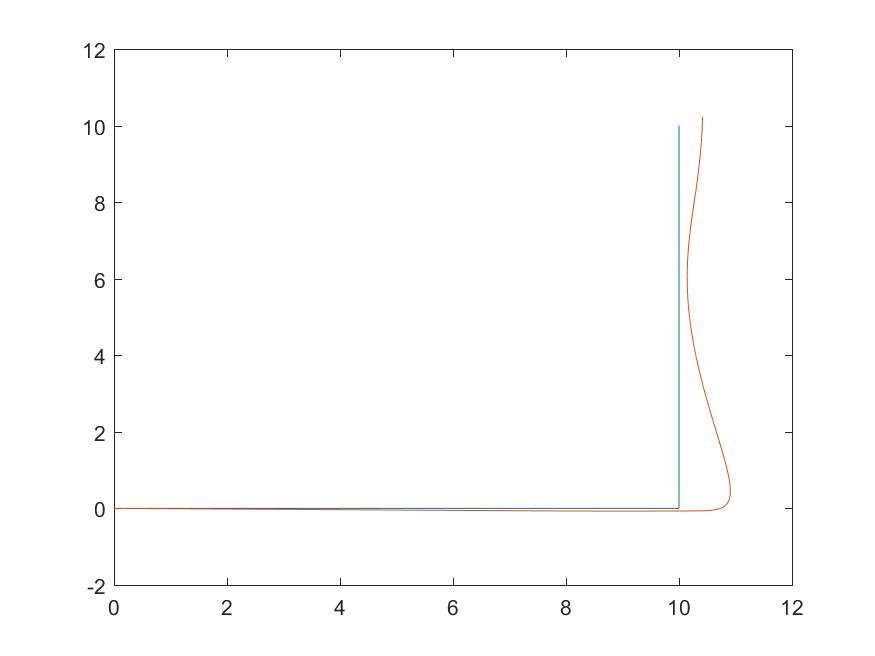
\includegraphics[scale=0.5]{Runge_kutta_comando_base_0001.jpg}
    {\footnotesize Fonte: Elaborada pelo autor.}
    \label{fig:label}
\end{figure}

\ref{fig:label} figura
\subsection{Rapid Prototyping}

\subsection{Fused Deposition Modeling}
Fused Deposition Modeling (FDM) ou Fused Filament Fabrication 
(FFF) é uma tecnologia categorizada como MA onde um filamento 
de material é forçado dentro de uma câmara através, geralmente,
de rolos dentados onde em uma região específica esse material 
é liquefeito. Por conta da pressão criada pelo filamento 
adentrando a câmara, ainda no estado sólido como um pistão, 
o material liquefeito é extrudado através de um bocal, 
comumente fabricado de bronze. Então, o filamento liquefeito é 
depositado em uma plataforma de forma a percorrer a trajetória 
desejada utilizando mecanismos movidos de forma controlada, 
geralmente por motores de passos. O processo é repetido camada 
por camada, de forma que elas estejam apoiadas por camadas 
anteriores e a primeira camada continue fixa na plataforma ou 
cama, até que o processo finalize (TURNER et al., 2014) \cite{turner14}.

\subsection{Desenvolvimento acadêmico em FDM}
O trabalho de Vyavahare et al. (2020) \cite{vyavahare20} apresenta algumas 
características sobre o desenvolvimento científico sobre 
FDM ao longo dos anos, tendo como base 211 artigos diferentes 
de 1994 a 2020. É apresentado um grande salto no número de 
artigos publicados no tema em anos recentes (2015 a 2018) 
(Figura 1), com 56\% dos temas trabalhados em torno da 
otimização de parâmetros de impressão, acompanhado de 17\% de 
trabalhos relacionados a aplicações utilizando o processo FDM 
(Figura 2).

\section{Geração de comando}
A geração de comando é o processo que coordena a ativação dos 
atuadores, motores, dentre outros componentes de uma impressora. 
Ele recebe como base uma série de comandos que precisam ser 
interpretados e interpolados. Esse processo é responsável pelo 
controle de velocidade, aceleração dentre outras atividades que 
variam no tempo. O desenvolvimento científico nesta área 
aplicado a impressoras 3D FDM se deu em tempos recentes, 
sendo sua aplicação majoritária relacionada às máquinas de 
Controle Numérico Computadorizado (CNC).

\subsection{Look ahead}
No processo de impressão 3D são fornecidos para a impressora 
uma sequência de pontos no espaço e limitações de velocidade 
entre os mesmos. A velocidade nos pontos é compartilhada entre 
trajetos em sequência, o que torna considerá-los 
independentemente ineficiente, introduzindo aceleração e 
desaceleração desnecessária impactando negativamente no tempo 
de impressão e na qualidade da peça impressa.
O algoritmo Look Ahead procura manter o máximo de velocidade 
possível entre movimentos distintos, evitando acelerações e 
desacelerações desnecessárias, apesar de ser necessário um 
pré-processamento desses pontos que introduzem um custo 
computacional maior (YU et al. 2020) \cite{yu20}.

\subsection{Curvas de velocidade}

\section{Controle e Otimização}

\subsection{Espaço de Estados}

\subsection{Integradores numéricos}

\subsubsection{Euller}

\subsubsection{Runge Kutta}


\subsection{Feedforward}
Dentre os métodos de controle em aplicações FDM o Feedforward 
é o mais eficiênte dada as limitações de custo em impressoras 
3D comuns e é capaz de ter um impacto maior em sistemas 
conhecidos e sensíveis ao erro, onde buscam corrigir o erro 
antes que ele aconteça (RAMANI et al. 2020; DUAN et al. 2018) || \cite{ramani20}\cite{duan18}.

\subsection{Feedback}

\subsection{Objective Function Otimization}

\section{Aplicações de Controle Impressora 3D}

\subsection{Input Shaper}
Conhecendo a trajetória desejada e conhecendo características 
do sistema é possível computar os comandos fornecidos para 
calcular uma série de comandos, levando em consideração as 
características do sistema para que o comando de referência 
seja modificado de forma à trajetória final ser o mais próximo 
possível do comando de referência. Entretanto, ao invés de 
computar todo o comando de referência, é possível obter um 
comando modificado em tempo real através de um filtro. 
Uma das abordagens desse tipo de filtro de comando é o 
Input Shaper, onde variados Shapers são construídos levando 
em consideração diferentes objetivos e restrições 
\cite{singhose97}.
Essa abordagem vem sendo utilizada na comunidade Maker depois 
da patente ter perdido o vigor, e tem aprimorado a área como
um todo, empurrando os limites anteriores de velocidade e 
precisão.

\subsection{B-spline}

\subsection{Robust Filter}
